\documentclass{article}
\usepackage[a4paper, total={6in, 10in}]{geometry}
\usepackage{graphicx}

\title{Project 4 for PSYC 489}
\author{Bingjun Guo (bingjun3)}
\begin{document}
\maketitle

\section*{Part 1}
Epochs needed for the nets to succeed on classification are all plotted in this part. The criterion for all sets is to classify all samples in each set correctly. The maximum number of epochs is set to be 500. Net2 is in shape 10-6-4. All nets' parameters are randomized initially.
\subsection*{Set 1: Non-Overlapping Categories}
Both networks succeed in classifying, since this set is non-overlapping, which indicates perpendicular, and thus makes this set specifically easy to classify. It is found that learning rate and momentum are ``the larger, the better'' for net1. For net2, 
the best learning rate lies around 2, and the best momentum lies between 0 and 0.3. Under the best settings, it takes only 1 epoch for net1 and 3 or 4 epochs for net2 to reach the criterion.
\\Notes that for Part 1, all experiments on momentum are run under the best learning rate without momentum, with is 8 for net1 and 2.2 for net2. Moreover, momentum are limited between 0 and 1 to avoid explosion. For this set, parameters in net1 actually never explode.
\begin{figure}[!ht]
    \begin{minipage}{0.5\textwidth}
        \centering
        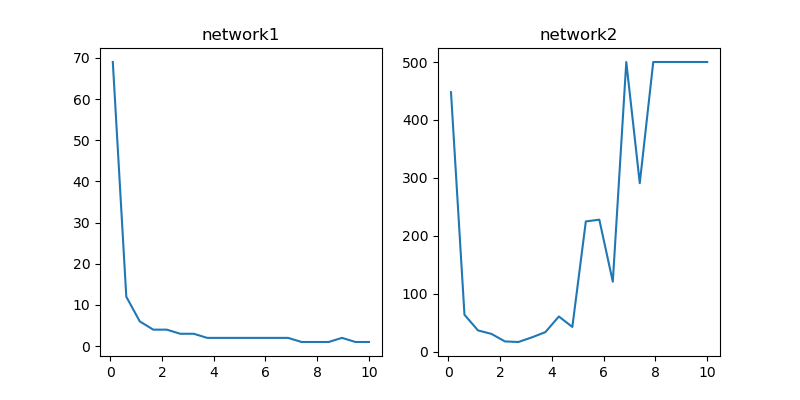
\includegraphics[width=\linewidth]{part1set1.png} 
        \caption{epochs v.s. learning rate (set 1)}   
    \end{minipage}\hfill
    \begin{minipage}{0.5\textwidth}
        \centering
        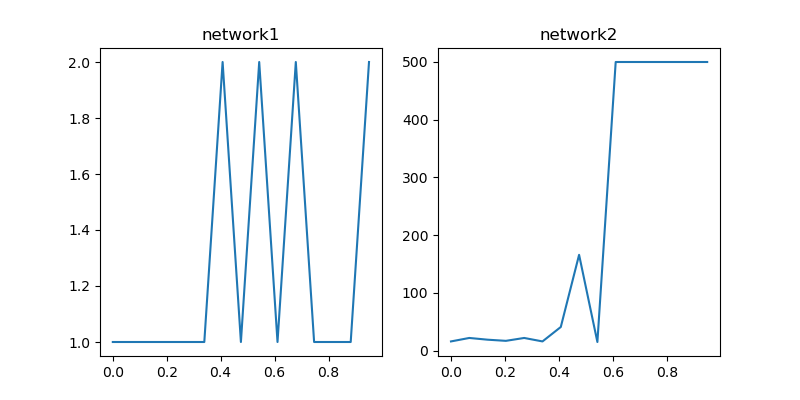
\includegraphics[width=\linewidth]{part1set1m.png}    
        \caption{epochs v.s. momentum (set 1)}
    \end{minipage}
\end{figure}

With noises, as is plotted below, the error rate for both nets will increase as the noise level increases. It can be indicated that net2 has stronger generalization capacity.
\begin{figure}[!ht]
    \centering
    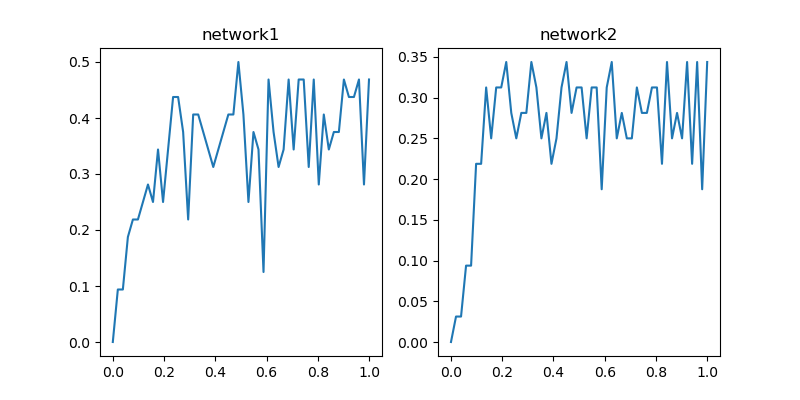
\includegraphics[width=0.5\textwidth]{part1set1g.png}
    \caption{error rate v.s. noise level (set 1)}
\end{figure}

\subsection*{Set 2: Linearly Separable Categories}
It seems that net1, which is simpler, fails to classify this set with larger learning rates, while net2 seems to occasionally fail on learning rates less than 20, and constantly fail on learning rates larger than 25. These can be caused by the dataset being more complex. Yet it is still linearly separable, it would be impossible to classify based on merely basic hyperplanes that are perpendicular to axis. For both nets, large momentum will lead to failure, and best momentum under the best learning rate is rather small for both nets. Under the best settings, it takes 1 or 2 epochs for net1 and 18 to 25 epochs for net2 to reach the criterion.
\begin{figure}[!ht]
    \begin{minipage}{0.5\textwidth}
        \centering
        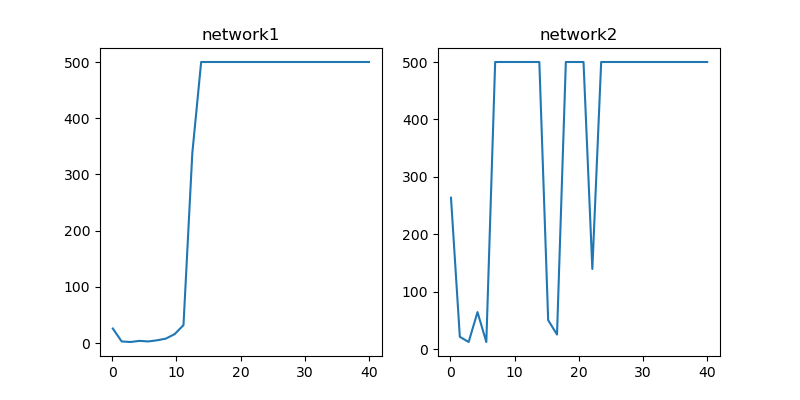
\includegraphics[width=\linewidth]{part1set2.png} 
        \caption{epochs v.s. learning rate (set 2)}   
    \end{minipage}\hfill
    \begin{minipage}{0.5\textwidth}
        \centering
        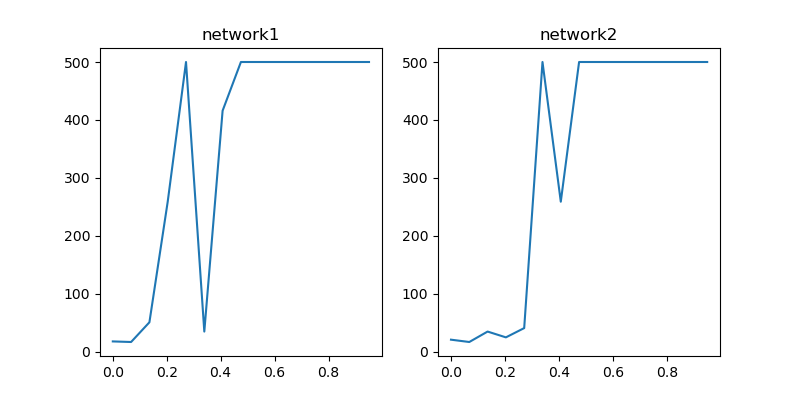
\includegraphics[width=\linewidth]{part1set2m.png}    
        \caption{epochs v.s. momentum (set 2)}
    \end{minipage}
\end{figure}

With noises, still, the error rate increases as noise level increases for both nets. However, the generalization capacities for both nets seem the same now.
\begin{figure}[!ht]
    \centering
    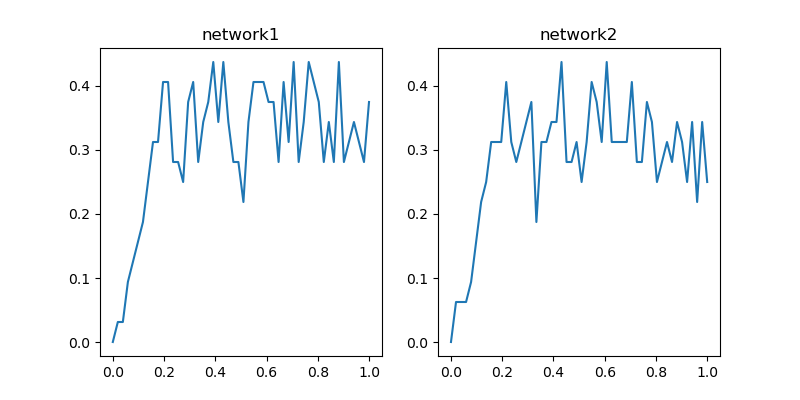
\includegraphics[width=0.5\textwidth]{part1set2g.png}
    \caption{error rate v.s. noise level (set 2)}
\end{figure}

\subsection*{Set 3: Non-Linearly Separable Categories}
Net1 fails to classify this set under any conditions, since single layer nets can only classify linearly separable data. Net2, as a two-layer net, succeed when learning rate is approximately between 0.5 and 19, under most of the momentum settings, taking $\approx50$ epochs.
\begin{figure}[!ht]
    \begin{minipage}{0.5\textwidth}
        \centering
        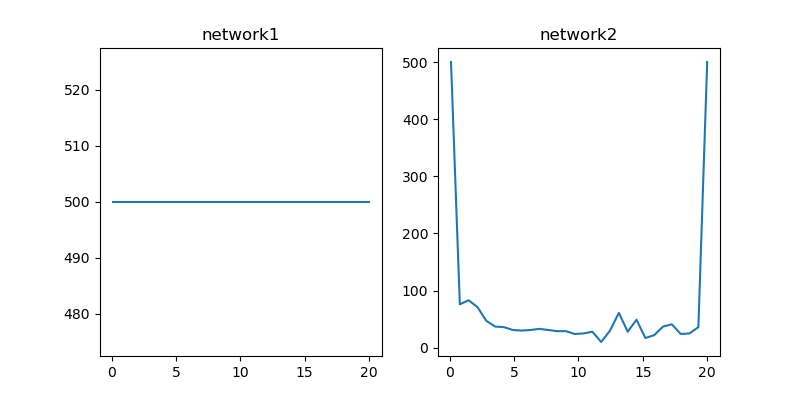
\includegraphics[width=\linewidth]{part1set3.png} 
        \caption{epochs v.s. learning rate (set 3)}   
    \end{minipage}\hfill
    \begin{minipage}{0.5\textwidth}
        \centering
        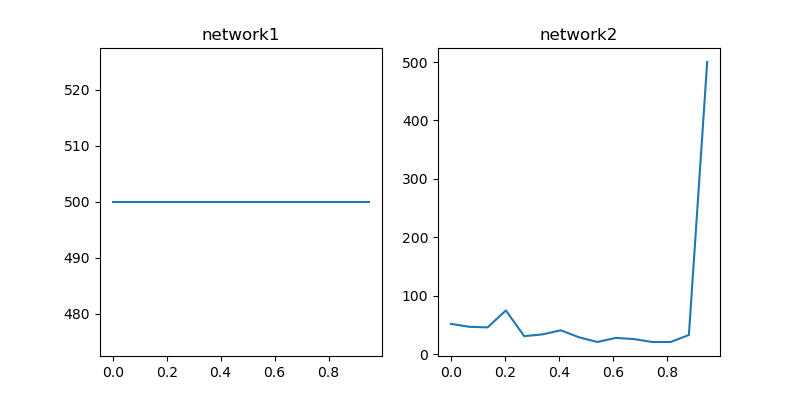
\includegraphics[width=\linewidth]{part1set3m.png}    
        \caption{epochs v.s. momentum (set 3)}
    \end{minipage}
\end{figure}

Since net1 fails on classifying this set, but its overall error rate somehow seems the same as that of net2 as noise gets larger. Moreover, the generalization capacity of net2 seems improved for a bit.
\begin{figure}[!ht]
    \centering
    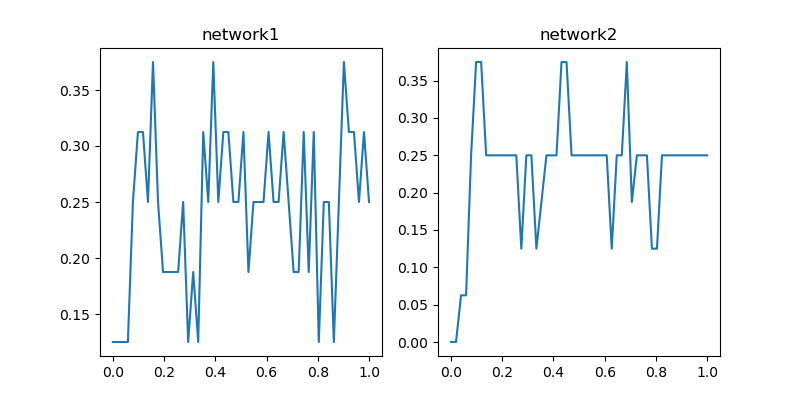
\includegraphics[width=0.5\textwidth]{part1set3g.png}
    \caption{error rate v.s. noise level (set 3)}
\end{figure}
\newpage

\section*{Part 2}
\subsection*{Part 2A}
Yes. It seems the training is fastest when learning rate is set to 6, which takes 7 to 15 epochs.
\subsection*{Part 2B}
The network gives $[0, 0, 0, 0, 0, 0, 0, 0]$. No. The network is still not able to generalize on this dataset, which can due to the limited training data. The network doesn't know the rule yet.
\subsection*{Part 2C}
Still with learning rate 6, it takes 6 to 12 epochs this time. The network was tested on patterns $[0, 0, 1, 1, 0, 0, 0, 0]$, $[1, 1, 0, 0, 0, 0, 1, 0]$, and $[0, 0, 1, 0, 0, 0, 0, 0]$, then produced $[0, 1, 0, 0, 0, 0, 0, 0]$, $[1, 1, 1, 0, 0, 0, 0, 0]$, and $[1, 1, 1, 0, 0, 0, 0, 0]$ as outputs. None of them is correct. The network still fails to generalize to untrained patterns, and it still doesn't know the rule. This may be caused by the limited learning capacity of the network.
\subsection*{Part3, Rules}
The output is $[0, 0, 0, 0, 0, 0, 0, 0]$ in most cases. The network seems always fail to generalize. The additional training seems not helping. It even forgets the training patterns in Part 2A. 
\end{document}
